% !TEX root = ../main.tex
\chapter{Resultados complementarios de segmentación}
\label{app:tejido-complementario}

Este apéndice completa los resultados de segmentación de WSI a resolución de
parche. Todos los modelos se evaluaron sobre las mismas \(31\,572\) celdas
de 23 WSI, con soportes de \(21\,796\) para tumor, \(8\,500\) para estroma
y \(1\,276\) para necrosis. Las tablas y matrices conservan los resultados
de cada presupuesto de etiquetas; el presupuesto completo se presenta en las
Tablas~\ref{tab:tejido-metricas-secundarias} y
\ref{tab:tejido-clases-completo}, y en la
Figura~\ref{fig:tejido-confusion-completo} del capítulo de resultados.

\section{Resultados por clase}

Las Tablas~\ref{tab:tejido-clases-250-500} y
\ref{tab:tejido-clases-1000-2500} presentan precisión, sensibilidad y F1 de
los cuatro presupuestos menores. La precisión indica qué proporción de las
predicciones de una clase corresponde a ella; la sensibilidad indica qué
proporción de las celdas de referencia de esa clase fue recuperada. F1 combina
ambas mediante su media armónica. El soporte conserva el número de celdas de
referencia y permite interpretar las diferencias entre clases.

\begin{table}[htbp]
    \centering
    \caption[Resultados por clase: presupuestos 250 y 500.]{Resultados por clase con \(250\) y \(500\) etiquetas por clase. Los soportes son los mismos para todos los modelos y presupuestos.}
    \label{tab:tejido-clases-250-500}
    \small
    \begin{tabular}{@{}rllrrrr@{}}
        \toprule
        Etiquetas/clase & Modelo & Clase & Precisión & Sensibilidad & F1 & Soporte \\
        \midrule
        \(250\) & VAE base & Tumor & 0,881 & 0,636 & 0,739 & \(21\,796\) \\
        \(250\) & VAE base & Estroma & 0,418 & 0,612 & 0,497 & \(8\,500\) \\
        \(250\) & VAE base & Necrosis & 0,198 & 0,527 & 0,288 & \(1\,276\) \\
        \(250\) & VAE-SO(2) & Tumor & 0,863 & 0,746 & 0,800 & \(21\,796\) \\
        \(250\) & VAE-SO(2) & Estroma & 0,494 & 0,517 & 0,505 & \(8\,500\) \\
        \(250\) & VAE-SO(2) & Necrosis & 0,175 & 0,526 & 0,263 & \(1\,276\) \\
        \(500\) & VAE base & Tumor & 0,873 & 0,687 & 0,769 & \(21\,796\) \\
        \(500\) & VAE base & Estroma & 0,446 & 0,532 & 0,485 & \(8\,500\) \\
        \(500\) & VAE base & Necrosis & 0,181 & 0,610 & 0,279 & \(1\,276\) \\
        \(500\) & VAE-SO(2) & Tumor & 0,888 & 0,697 & 0,781 & \(21\,796\) \\
        \(500\) & VAE-SO(2) & Estroma & 0,481 & 0,670 & 0,560 & \(8\,500\) \\
        \(500\) & VAE-SO(2) & Necrosis & 0,285 & 0,589 & 0,384 & \(1\,276\) \\
        \bottomrule
    \end{tabular}
\end{table}

\begin{table}[htbp]
    \centering
    \caption[Resultados por clase: presupuestos 1000 y 2500.]{Resultados por clase con \(1\,000\) y \(2\,500\) etiquetas por clase. Los soportes son los mismos para todos los modelos y presupuestos.}
    \label{tab:tejido-clases-1000-2500}
    \small
    \begin{tabular}{@{}rllrrrr@{}}
        \toprule
        Etiquetas/clase & Modelo & Clase & Precisión & Sensibilidad & F1 & Soporte \\
        \midrule
        \(1\,000\) & VAE base & Tumor & 0,878 & 0,674 & 0,763 & \(21\,796\) \\
        \(1\,000\) & VAE base & Estroma & 0,487 & 0,658 & 0,560 & \(8\,500\) \\
        \(1\,000\) & VAE base & Necrosis & 0,292 & 0,770 & 0,424 & \(1\,276\) \\
        \(1\,000\) & VAE-SO(2) & Tumor & 0,886 & 0,763 & 0,820 & \(21\,796\) \\
        \(1\,000\) & VAE-SO(2) & Estroma & 0,549 & 0,612 & 0,578 & \(8\,500\) \\
        \(1\,000\) & VAE-SO(2) & Necrosis & 0,274 & 0,710 & 0,395 & \(1\,276\) \\
        \(2\,500\) & VAE base & Tumor & 0,899 & 0,792 & 0,842 & \(21\,796\) \\
        \(2\,500\) & VAE base & Estroma & 0,608 & 0,716 & 0,657 & \(8\,500\) \\
        \(2\,500\) & VAE base & Necrosis & 0,464 & 0,860 & 0,603 & \(1\,276\) \\
        \(2\,500\) & VAE-SO(2) & Tumor & 0,903 & 0,823 & 0,861 & \(21\,796\) \\
        \(2\,500\) & VAE-SO(2) & Estroma & 0,621 & 0,738 & 0,675 & \(8\,500\) \\
        \(2\,500\) & VAE-SO(2) & Necrosis & 0,542 & 0,685 & 0,605 & \(1\,276\) \\
        \bottomrule
    \end{tabular}
\end{table}


\clearpage

\section{Intervalos de las métricas secundarias}

La Tabla~\ref{tab:tejido-secundarias-intervalos} presenta los intervalos
percentiles de las diferencias de exactitud, exactitud balanceada y entropía
cruzada. Se calcularon con \(10\,000\) réplicas de bootstrap pareado,
estratificado por el soporte de tejido de las WSI, con semilla 3901. Una
diferencia positiva favorece al VAE base en exactitud y exactitud balanceada;
en entropía cruzada, una diferencia negativa favorece a esa rama. Los
intervalos son puntuales y exploratorios. La familia primaria de macro-F1 y
área bajo la curva mantiene los intervalos simultáneos descritos en
metodología.

\begin{table}[htbp]
    \centering
    \caption[Diferencias e intervalos exploratorios de métricas secundarias.]{Diferencias VAE base menos VAE-\(\mathrm{SO}(2)\) e intervalos percentiles puntuales del 95\% para métricas secundarias. Se obtuvieron con el mismo bootstrap pareado y estratificado por WSI de la comparación primaria. Son intervalos exploratorios sin ajuste simultáneo.}
    \label{tab:tejido-secundarias-intervalos}
    \small
    \begin{tabular}{@{}rlrr@{}}
        \toprule
        Etiquetas/clase & Métrica & Diferencia & IC puntual 95\% \\
        \midrule
        \(250\) & Exactitud & \(-0,050\) & \([-0,085;-0,021]\) \\
        \(250\) & Exactitud balanceada & \(-0,005\) & \([-0,039;0,025]\) \\
        \(250\) & Entropía cruzada & \(0,051\) & \([0,009;0,093]\) \\
        \(500\) & Exactitud & \(-0,044\) & \([-0,075;-0,009]\) \\
        \(500\) & Exactitud balanceada & \(-0,043\) & \([-0,096;0,021]\) \\
        \(500\) & Entropía cruzada & \(0,088\) & \([0,016;0,150]\) \\
        \(1\,000\) & Exactitud & \(-0,047\) & \([-0,077;-0,019]\) \\
        \(1\,000\) & Exactitud balanceada & \(0,006\) & \([-0,027;0,043]\) \\
        \(1\,000\) & Entropía cruzada & \(0,454\) & \([0,293;0,634]\) \\
        \(2\,500\) & Exactitud & \(-0,020\) & \([-0,043;0,001]\) \\
        \(2\,500\) & Exactitud balanceada & \(0,040\) & \([-0,002;0,098]\) \\
        \(2\,500\) & Entropía cruzada & \(0,121\) & \([0,044;0,205]\) \\
        \(5\,671\) & Exactitud & \(0,013\) & \([-0,009;0,035]\) \\
        \(5\,671\) & Exactitud balanceada & \(0,024\) & \([0,005;0,045]\) \\
        \(5\,671\) & Entropía cruzada & \(-0,189\) & \([-0,345;-0,066]\) \\
        \bottomrule
    \end{tabular}
\end{table}


\clearpage

\section{Matrices de confusión}

Las Figuras~\ref{fig:tejido-confusion-250},
\ref{fig:tejido-confusion-500}, \ref{fig:tejido-confusion-1000} y
\ref{fig:tejido-confusion-2500} muestran ambos modelos en los cuatro
presupuestos menores. Cada fila corresponde a la clase de referencia y cada
columna a la clase predicha. Se presentan el conteo y el porcentaje de la
fila, usando una escala de color común de 0 a 100\%. Así se pueden comparar
las proporciones de aciertos y las confusiones aun cuando las clases tengan
soportes distintos.

\begin{figure}[htbp]
    \centering
    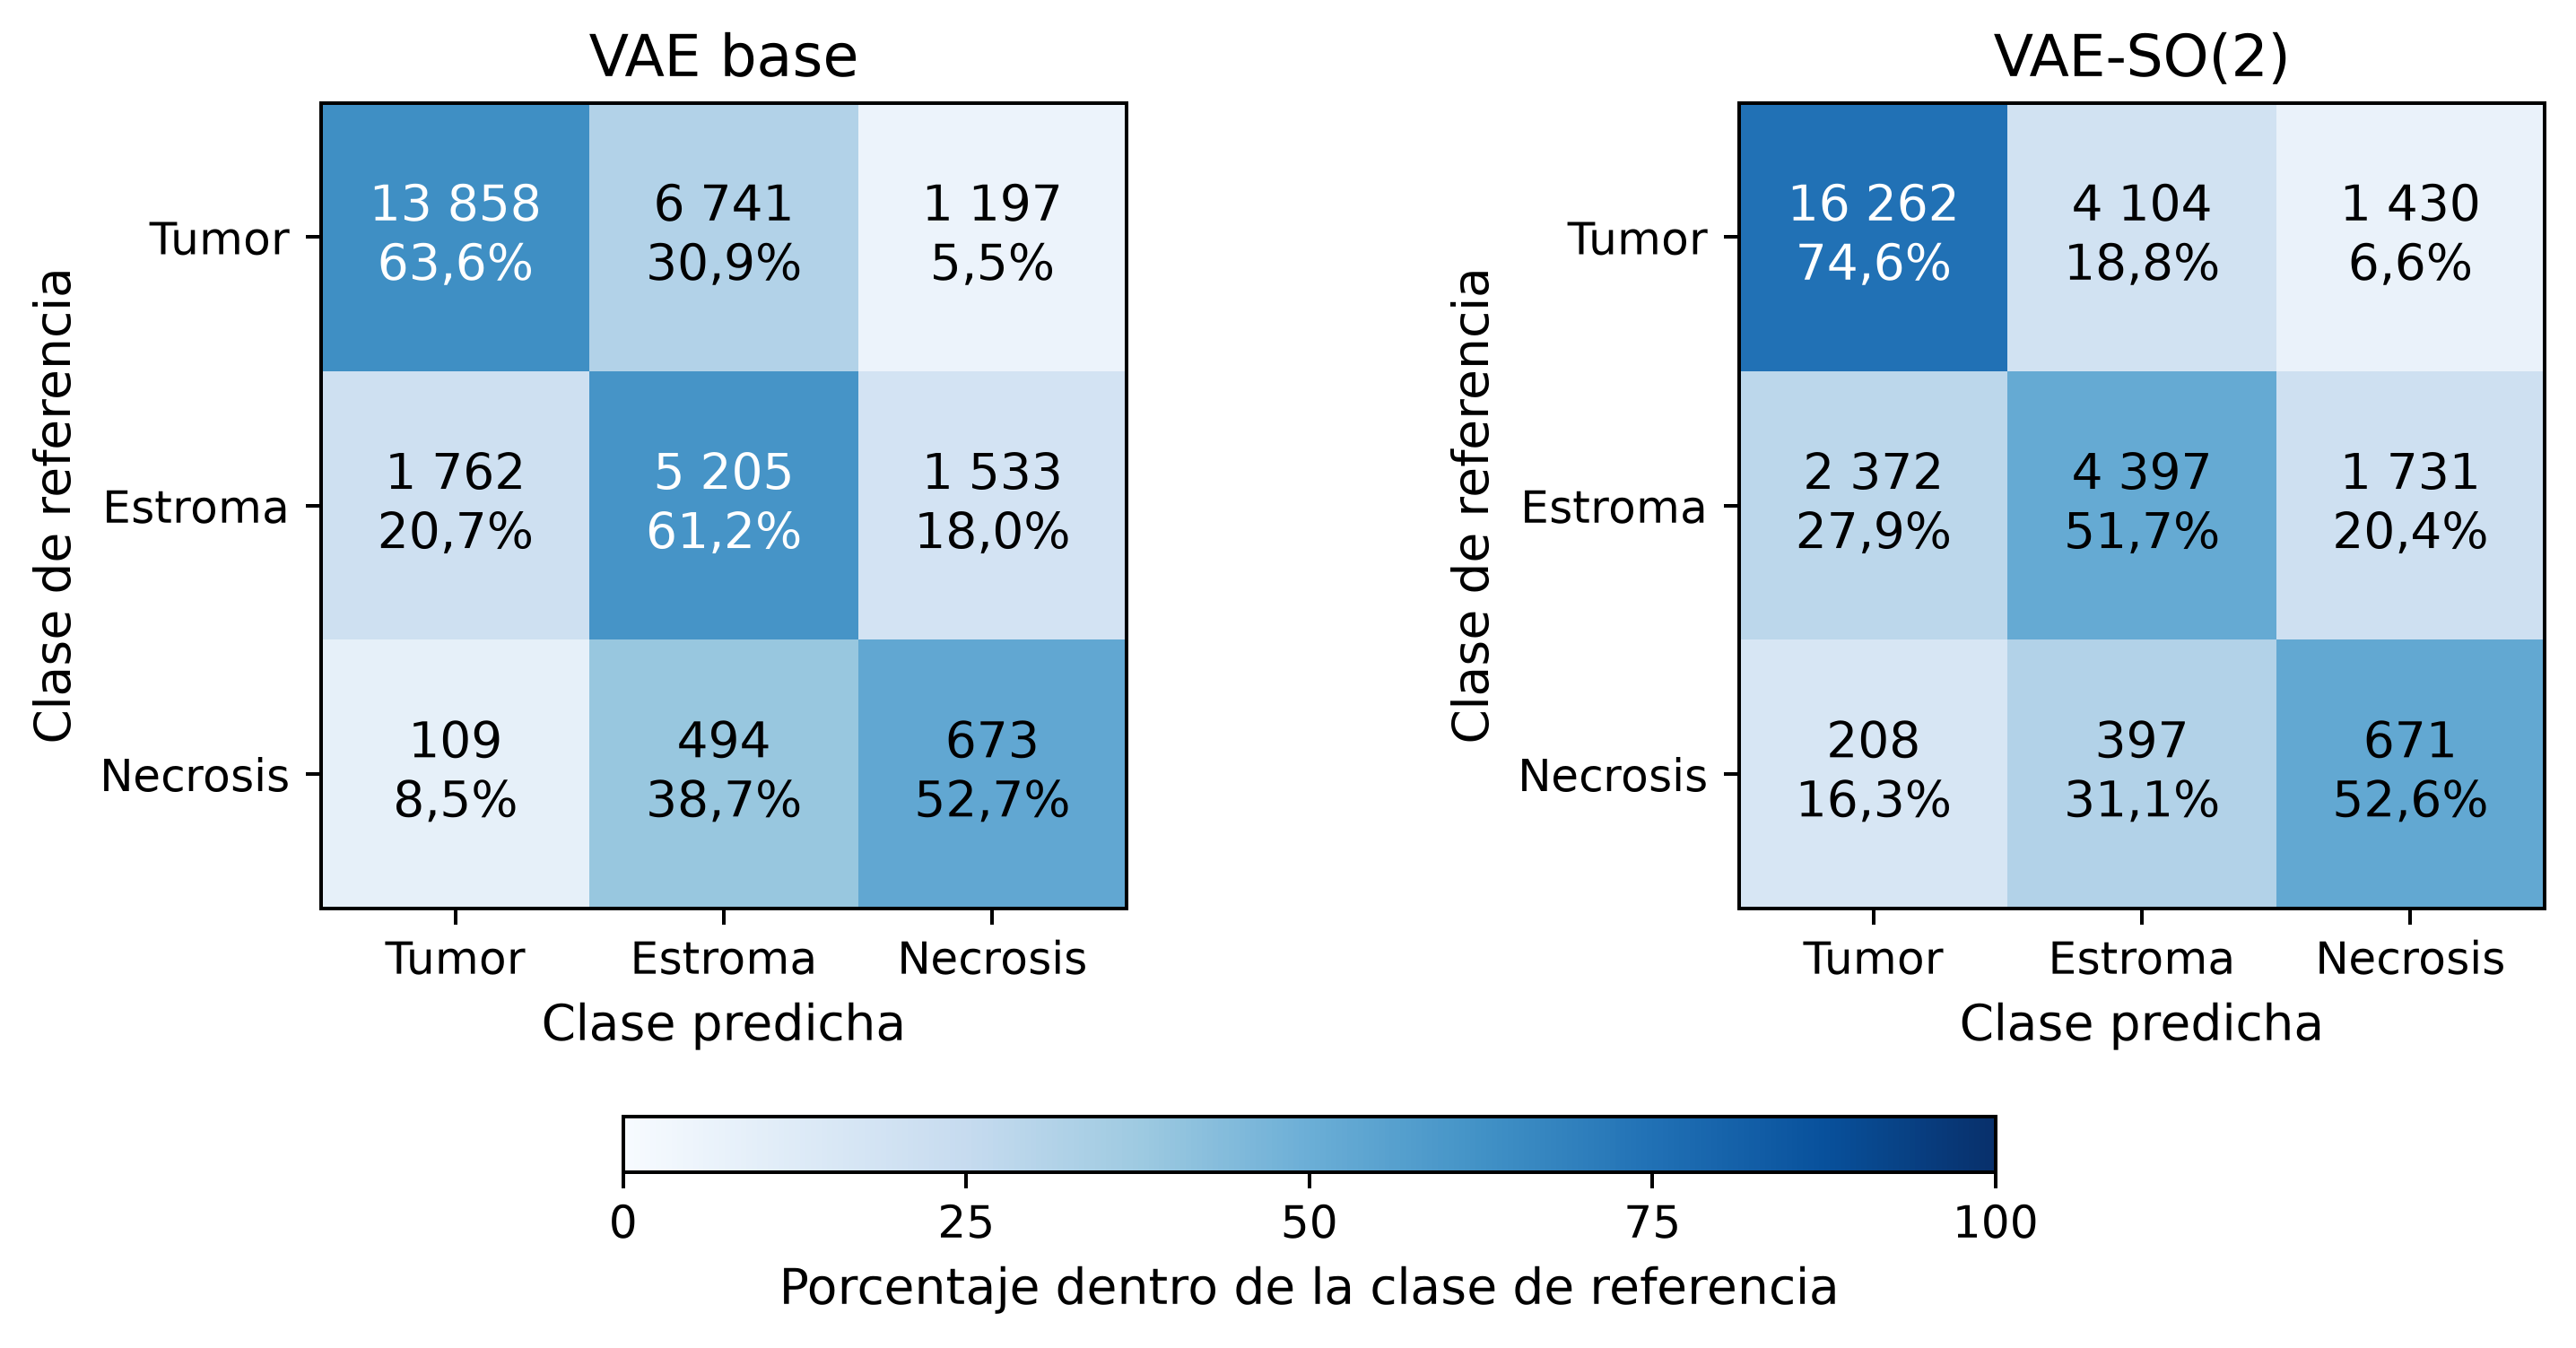
\includegraphics[width=\textwidth]{tissue_confusion_budget_250.png}
    \caption[Matrices de confusión de tejido: 250 etiquetas por clase.]{Matrices
    de confusión de segmentación con 250 etiquetas por clase. Conteos y
    porcentajes dentro de la clase de referencia, sobre las mismas celdas de
    prueba en ambas ramas.}
    \label{fig:tejido-confusion-250}
\end{figure}

\begin{figure}[p]
    \centering
    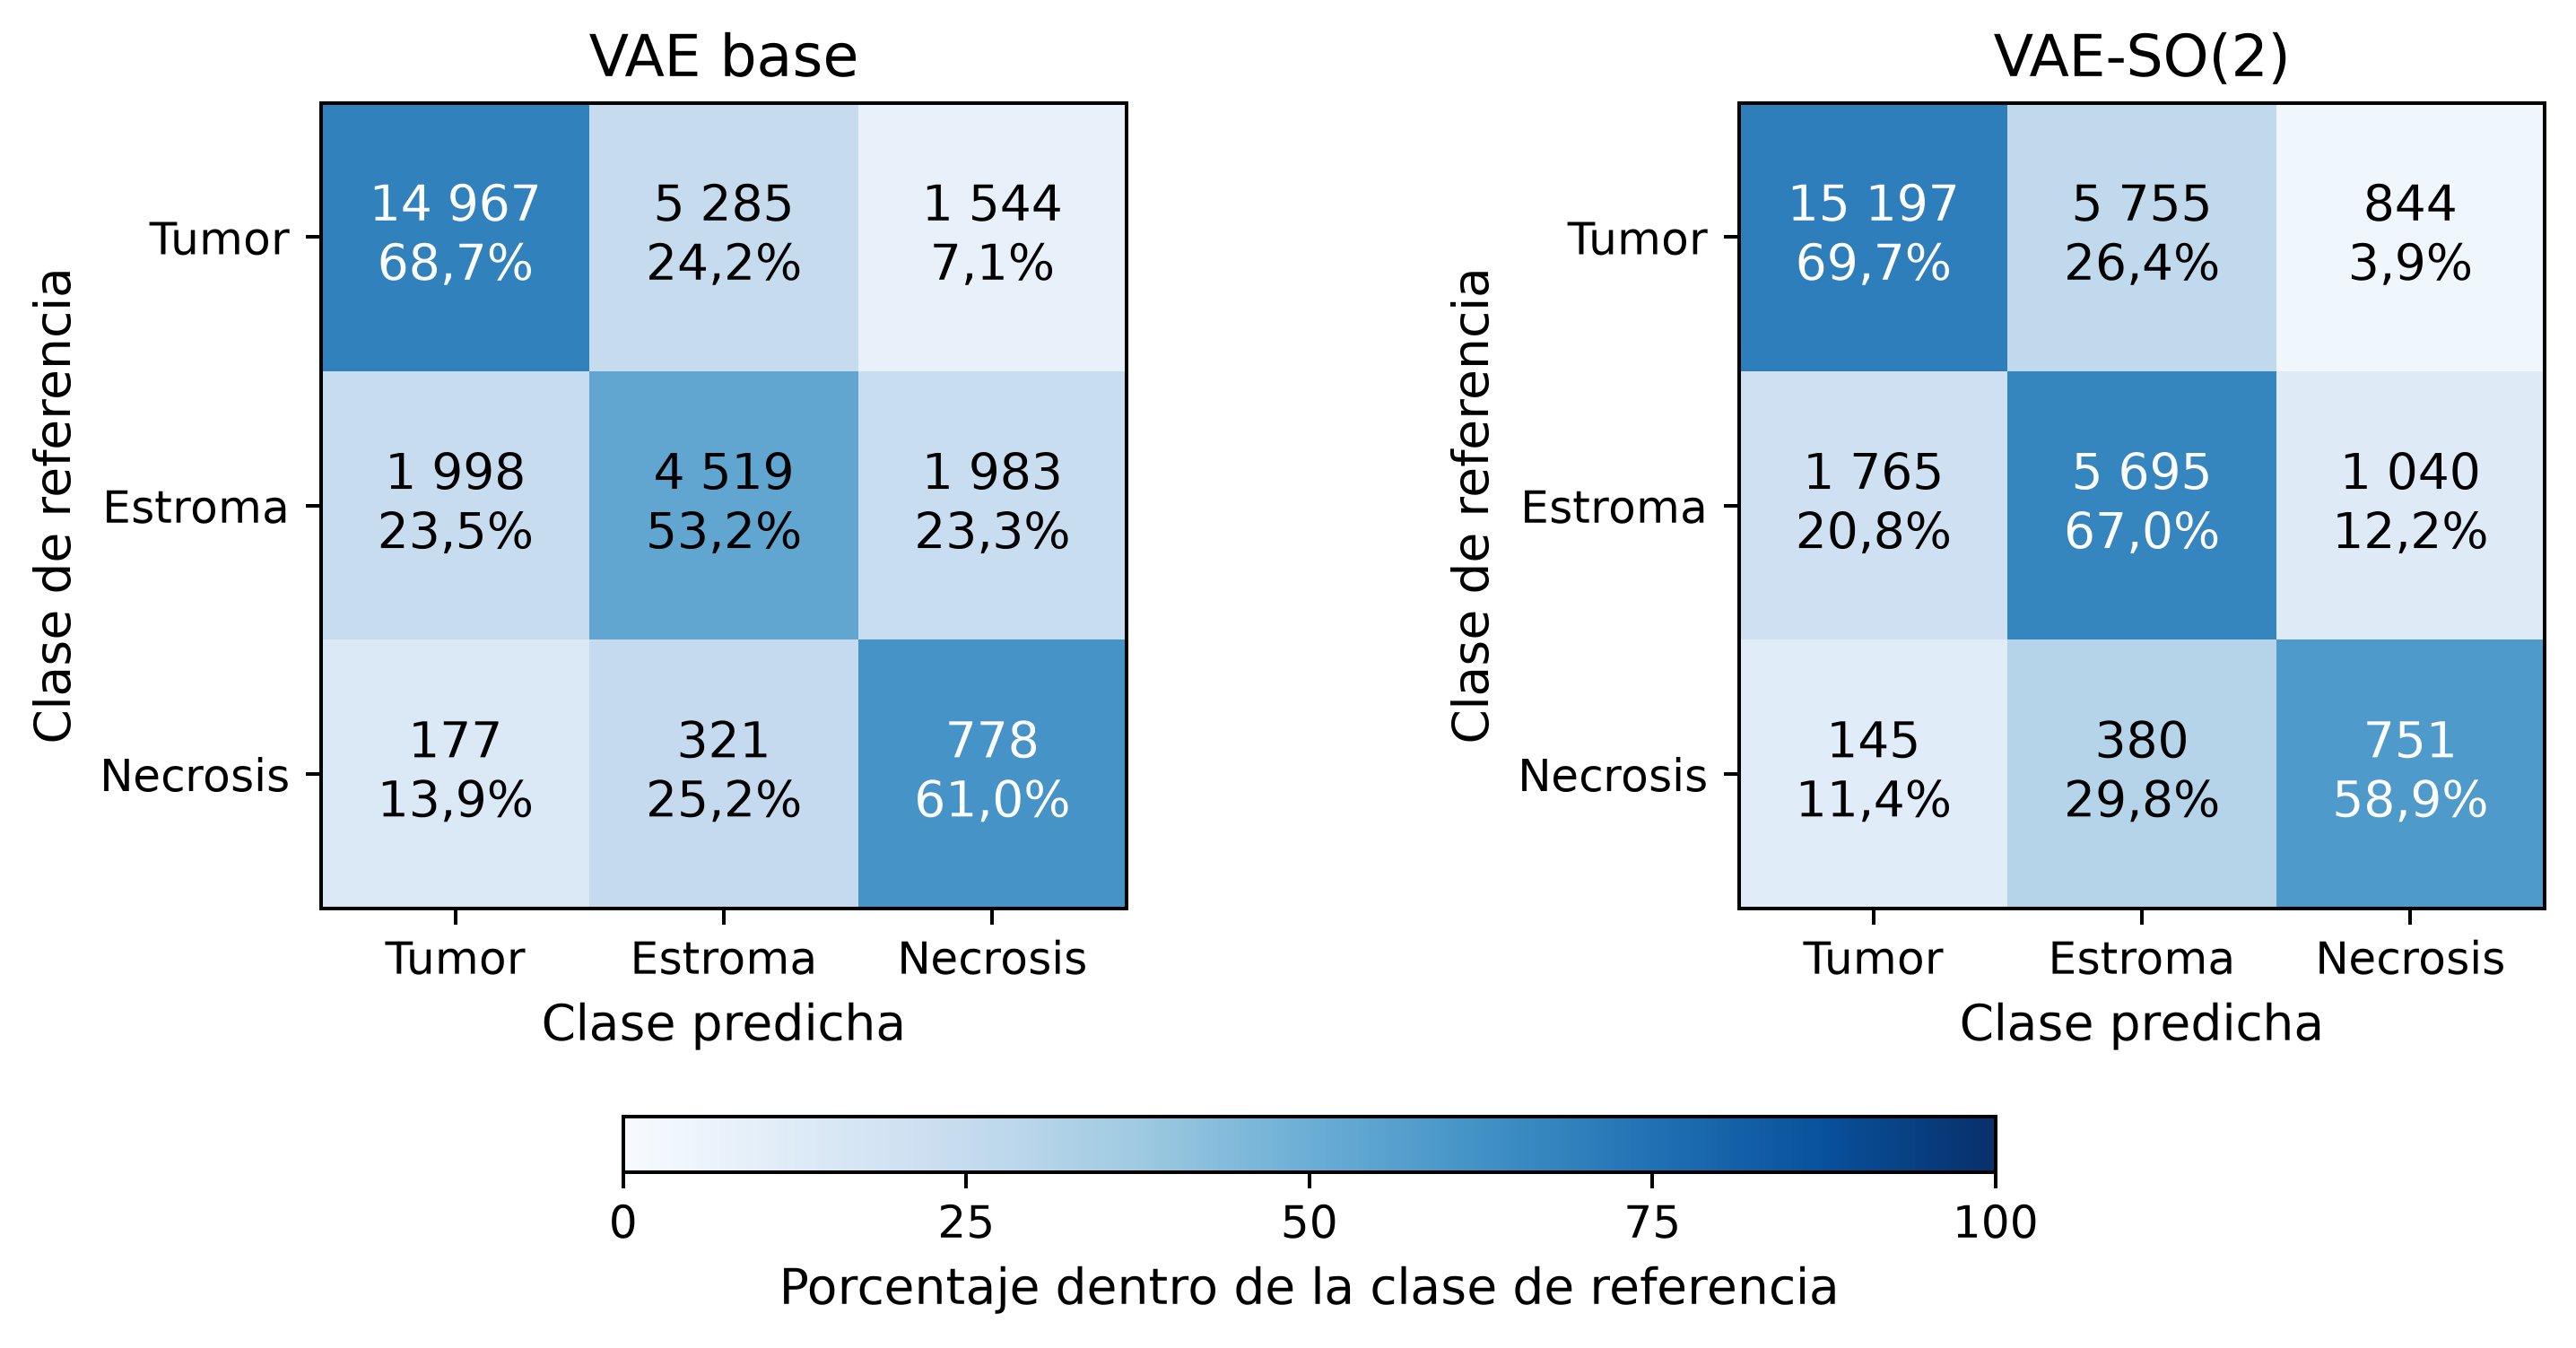
\includegraphics[width=\textwidth]{tissue_confusion_budget_500.png}
    \caption[Matrices de confusión de tejido: 500 etiquetas por clase.]{Matrices
    de confusión de segmentación con 500 etiquetas por clase. Conteos y
    porcentajes dentro de la clase de referencia.}
    \label{fig:tejido-confusion-500}
\end{figure}

\begin{figure}[p]
    \centering
    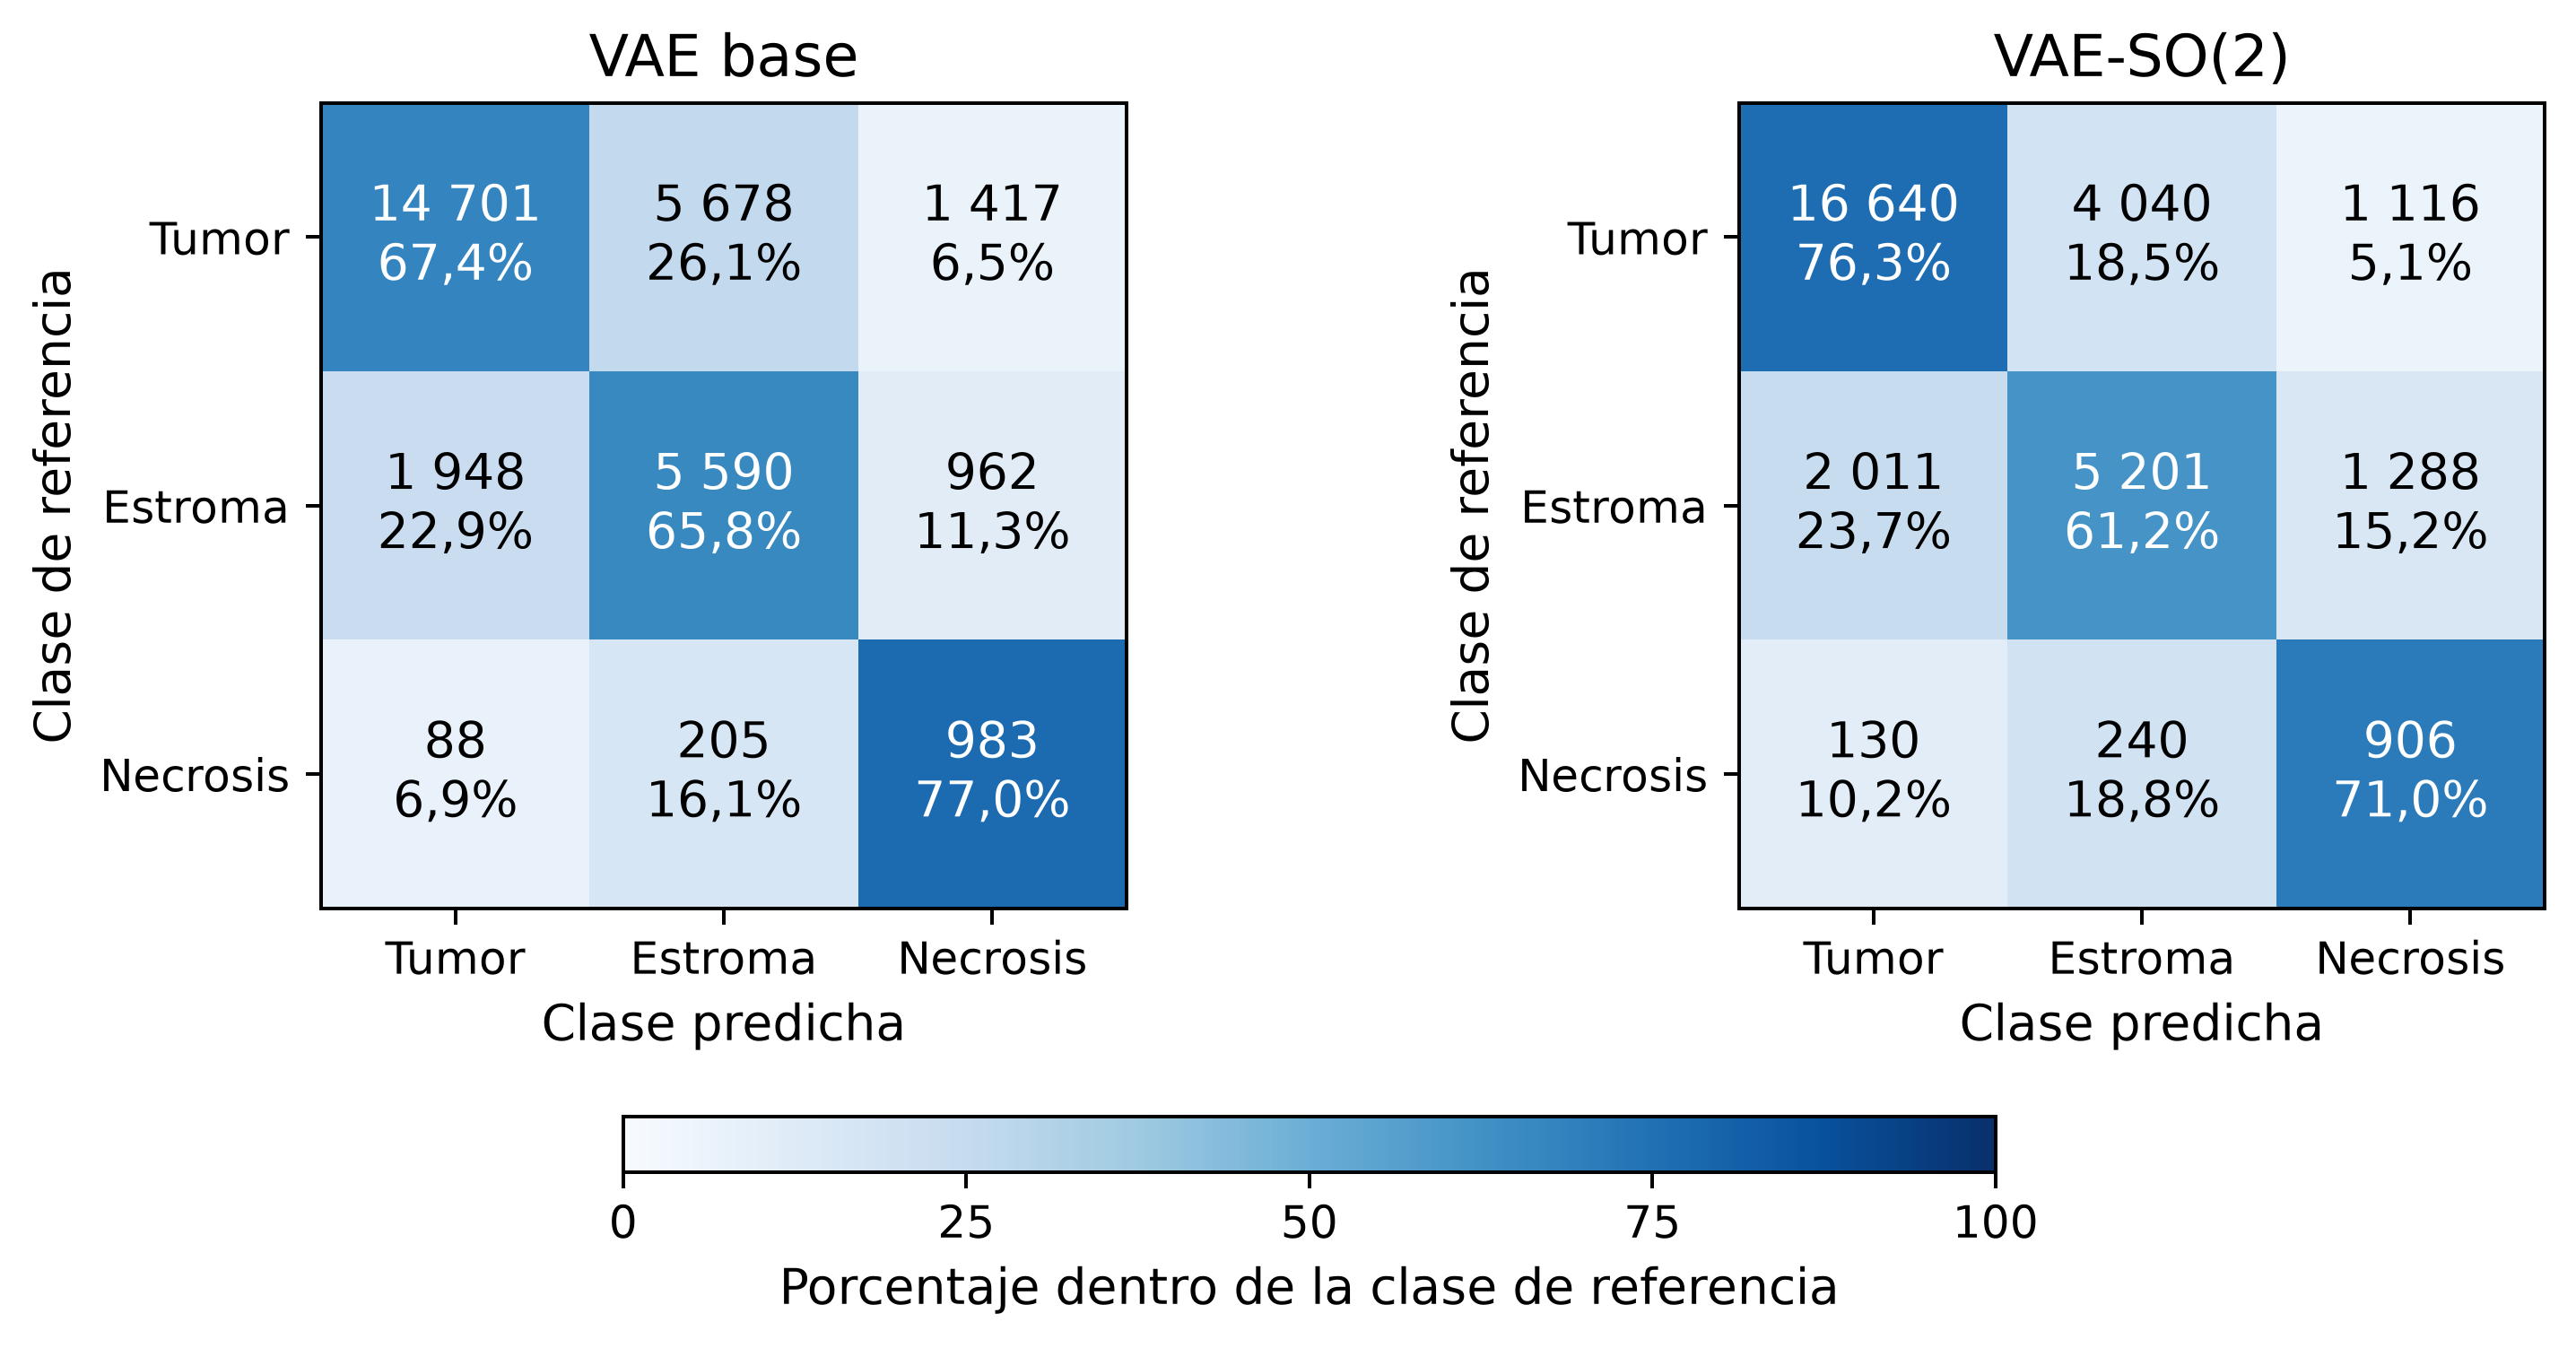
\includegraphics[width=\textwidth]{tissue_confusion_budget_1000.png}
    \caption[Matrices de confusión de tejido: 1 000 etiquetas por clase.]{Matrices
    de confusión de segmentación con \(1\,000\) etiquetas por clase. Conteos y
    porcentajes dentro de la clase de referencia.}
    \label{fig:tejido-confusion-1000}
\end{figure}

\begin{figure}[p]
    \centering
    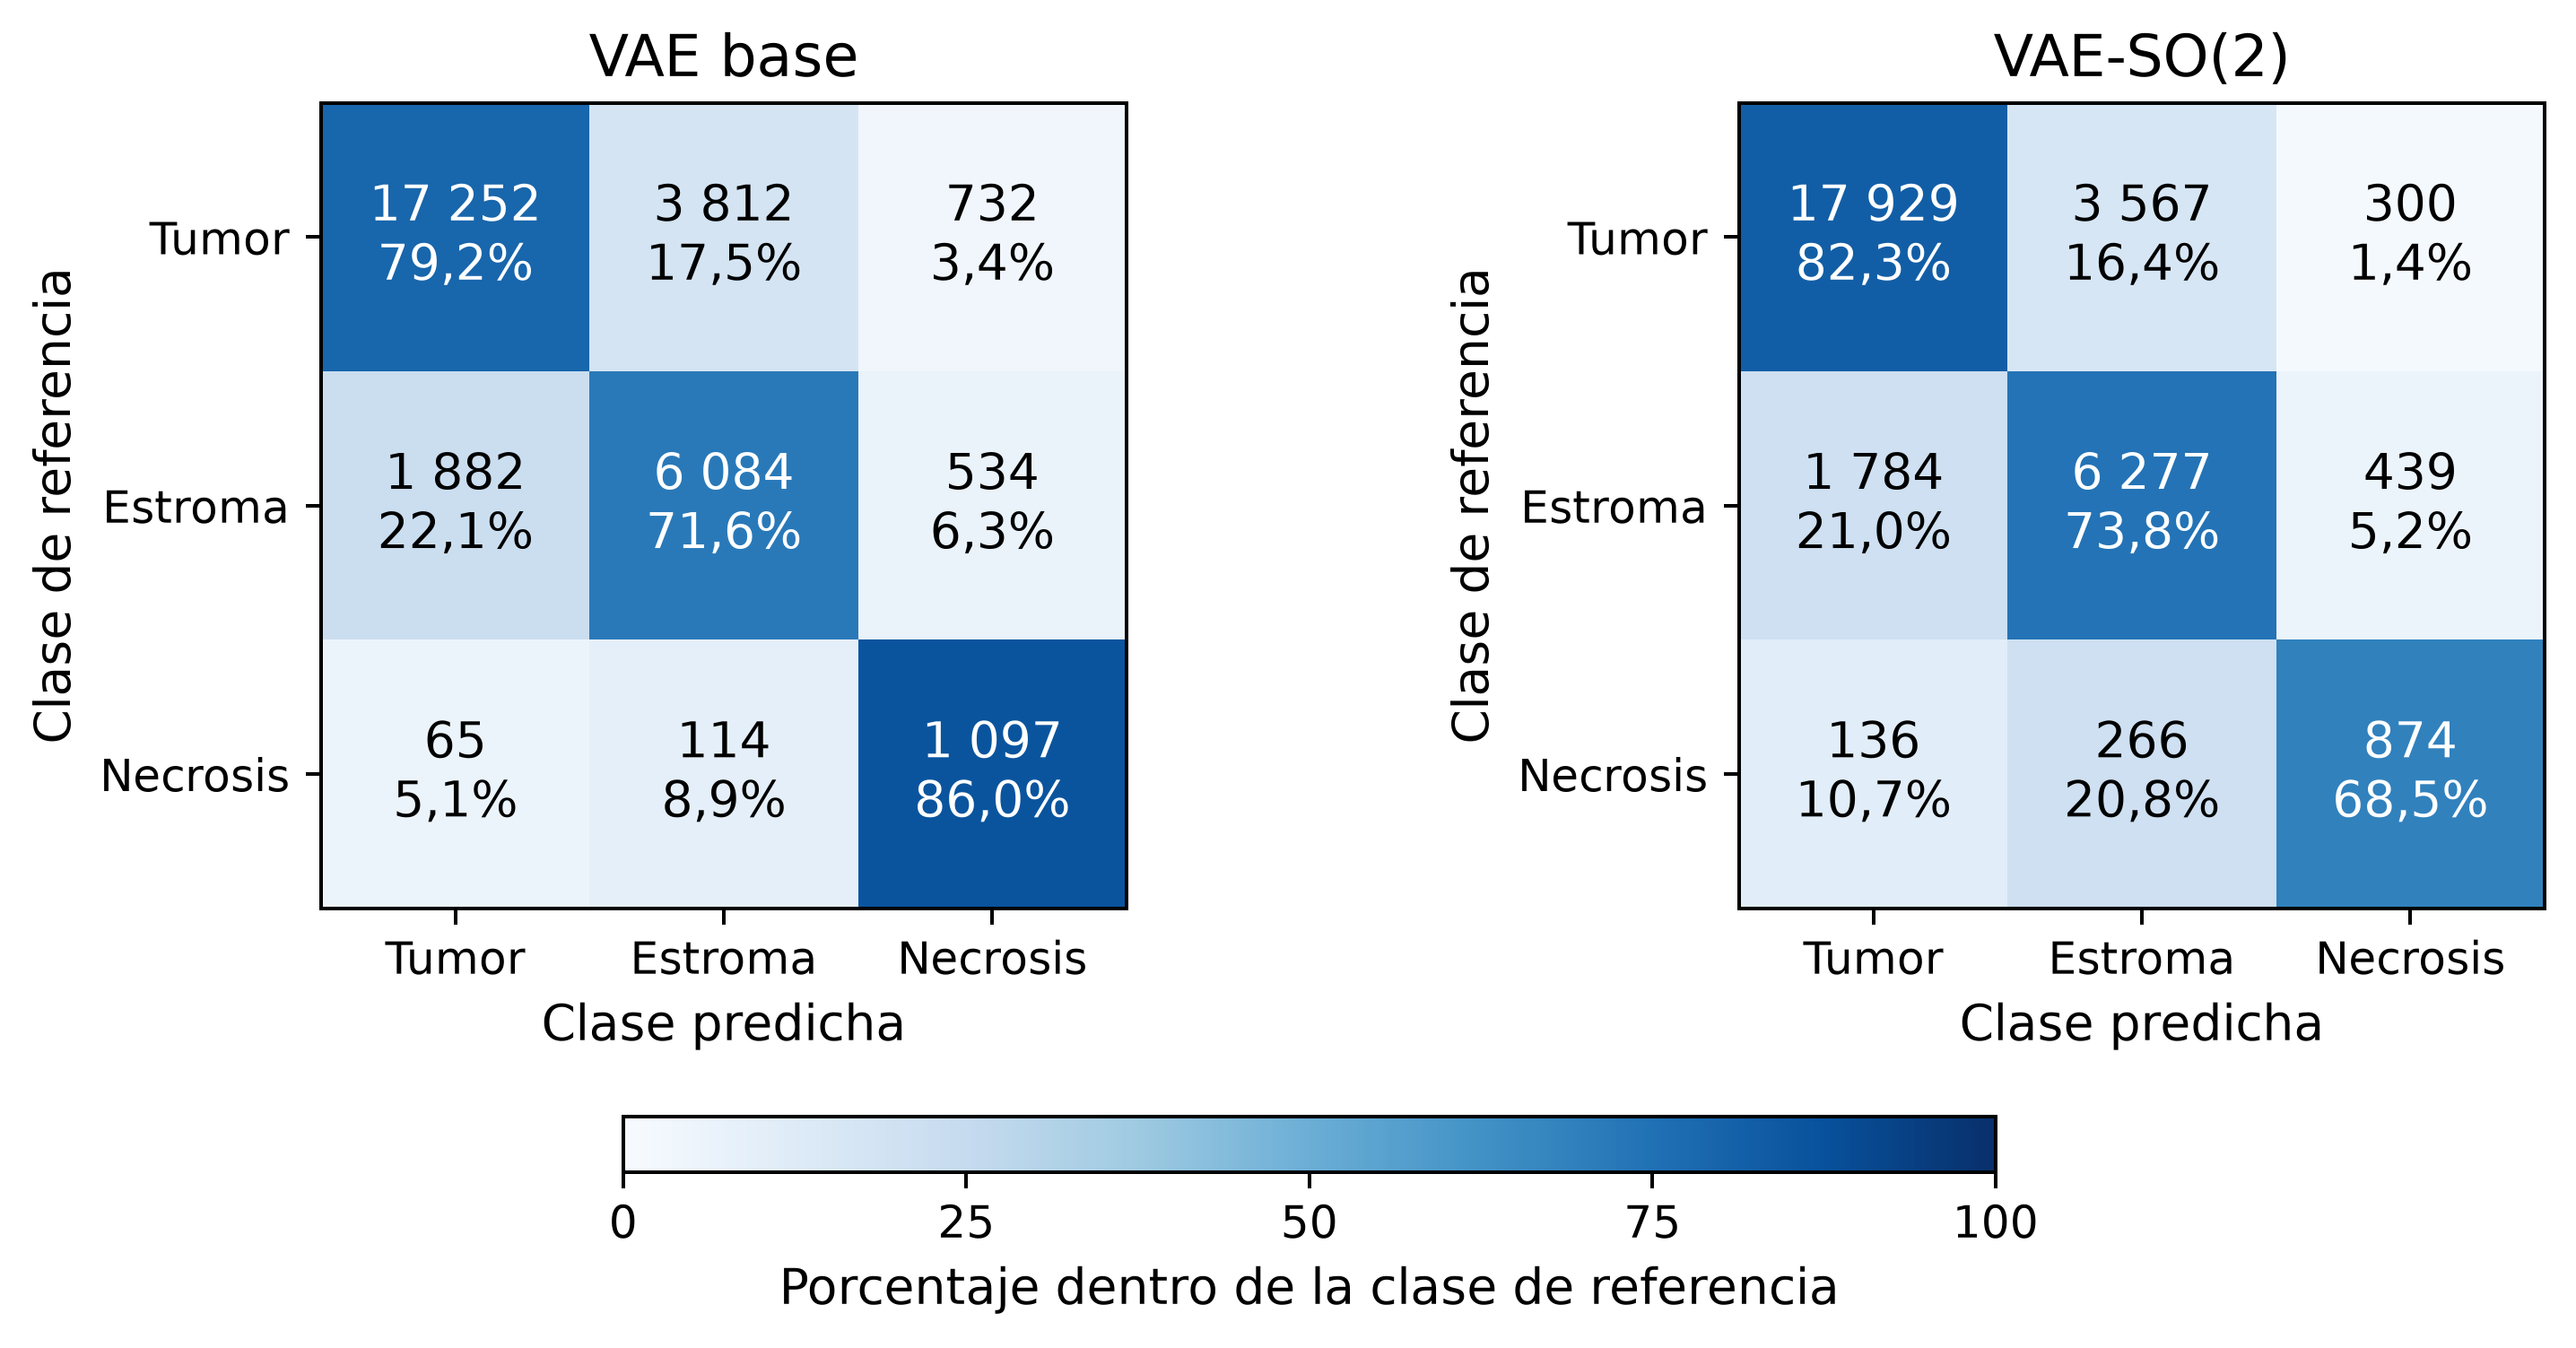
\includegraphics[width=\textwidth]{tissue_confusion_budget_2500.png}
    \caption[Matrices de confusión de tejido: 2 500 etiquetas por clase.]{Matrices
    de confusión de segmentación con \(2\,500\) etiquetas por clase. Conteos y
    porcentajes dentro de la clase de referencia.}
    \label{fig:tejido-confusion-2500}
\end{figure}
